\documentclass[12pt, twoside]{article}
\usepackage[letterpaper, margin=1in, headsep=0.5in]{geometry}
\usepackage[english]{babel}
\usepackage[utf8]{inputenc}
\usepackage{amsmath}
\usepackage{amsfonts}
\usepackage{amssymb}
\usepackage{tikz}
\usetikzlibrary{quotes, angles}
\usepackage{graphicx}
\usepackage{enumitem}
\usepackage{multicol}

\newif\ifmeta
\metatrue %print standards and topics tags

\title{Regents Geometry}
\author{Chris Huson}
\date{September 2020}

\usepackage{fancyhdr}
\pagestyle{fancy}
\fancyhf{}
\renewcommand{\headrulewidth}{0pt} % disable the underline of the header
\raggedbottom


\fancyhead[LE]{\thepage}
\fancyhead[RO]{\thepage \\ Name: \hspace{4cm} \,\\}
\fancyhead[LO]{BECA / Dr. Huson / Geometry 10-Trig+similarity+analytics\\* pset ID: 166}

\begin{document}

\subsubsection*{10-1bDN-Trig}
\begin{enumerate}
\item A dilation centered at the origin with scale factor $k=\frac{1}{2}$ maps $\overleftrightarrow{AB} \rightarrow \overleftrightarrow{A'B'}$. 
\begin{multicols}{2}
\begin{enumerate}
  \item Draw and label the image.
  \item What are the $y$-intercepts of $\overleftrightarrow{A'B'}$ and $\overleftrightarrow{AB}$?
  \item What are their slopes?
  \item Write down the equations of the two lines.
  \begin{flushright}
    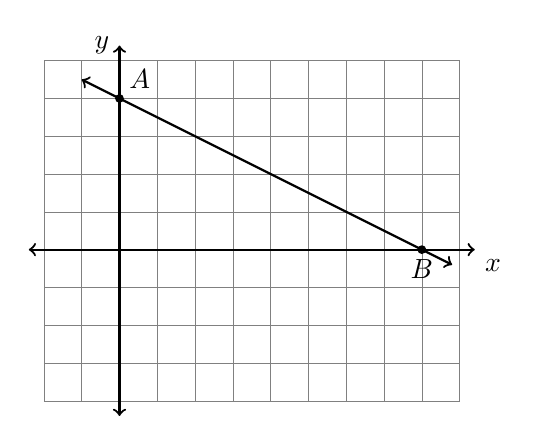
\begin{tikzpicture}[scale=.48]
      \draw [help lines] (-2,-4) grid (9,5);
      \draw [thick, <->] (-2.4,0) -- (9.4,0) node [below right] {$x$};
      \draw [thick, <->] (0,-4.4)--(0,5.4) node [left] {$y$};
      \draw [thick, <->] (-1,4.5)--(8.8,-0.4);
      \draw [fill] (0,4) circle [radius=0.1] node[above right] {$A$};
      \draw [fill] (8,0) circle [radius=0.1] node[below] {$B$};
    \end{tikzpicture}
  \end{flushright}
\end{enumerate}
\end{multicols} \vspace{1cm}


\item A line through the point $A(2,-2)$ has a slope $m=\frac{1}{2}$. A dilation centered at the origin maps $A \rightarrow B$ as shown. Draw the image the line. Write the equations of both lines.
\begin{flushright} %4 quadrant regents grid w T-Chart
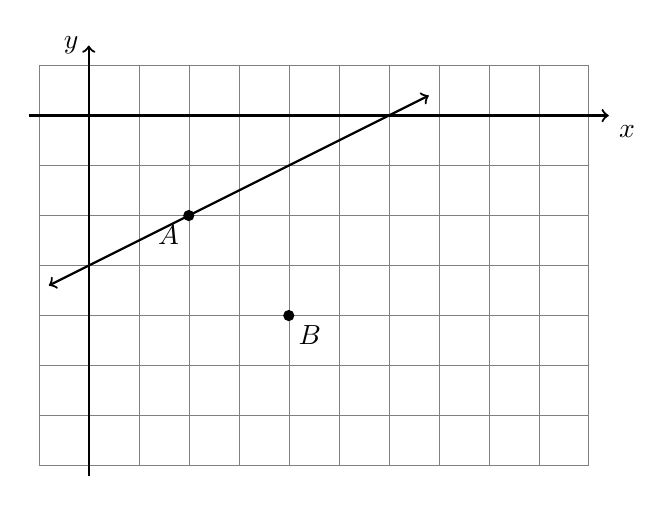
\begin{tikzpicture}[scale=.635]
  \draw [help lines] (-1,-7) grid (10,1);
  \draw [thick, ->] (-1.2,0) -- (10.4,0) node [below right] {$x$};
  \draw [thick, ->] (0,-7.2)--(0,1.4) node [left] {$y$};
  \draw [<->, thick] (-0.8,-3.4)--(6.8,0.4);
  \draw [fill] (2,-2) circle [radius=0.1]node[below left]{$A$};
  %\draw [fill] (3,0) circle [radius=0.1]node[below left]{$C$};
  \draw [fill] (4,-4) circle [radius=0.1]node[below right]{$B$};
\end{tikzpicture}
\end{flushright}


\item In $\triangle ABC$ shown below, $\angle ACB$ is a right angle, $E$ is a point on $\overline{AC}$, and $\overline{ED}$ is drawn perpendicular to leg $\overline{AC}$. If $AC = 8$, $BC = 6$, and $DE = 4$, what is the length of $\overline{AE}$? 
\begin{flushright}
  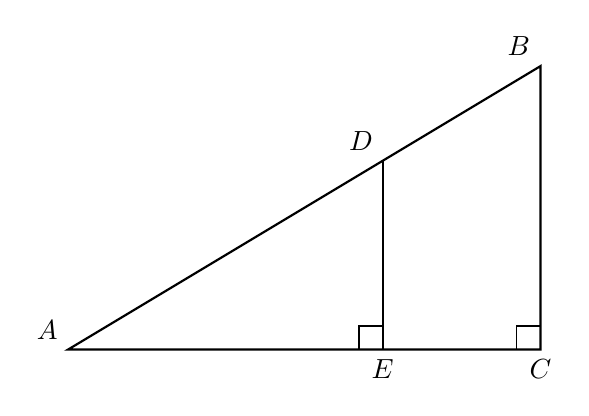
\begin{tikzpicture}[scale=0.6]
    \draw [-, thick] (0,0) node[above left]{$A$}--
    (10,0) node[below]{$C$}--
    (10,6) node[above left]{$B$}--cycle;
    \draw [thick] (6.66,0)--(6.66,4);
    \node at (6.66,0) [below]{$E$};
    \node at (6.66,4) [above left]{$D$};
    \draw (10,0) ++(-0.5,0)--++(0,0.5)--++(0.5,0);
    \draw (6.66,0) ++(-0.5,0)--++(0,0.5)--++(0.5,0);
    %\node at (4, 0) [below]{$12$};
    %\node at (3,2) [above]{$9$};
    %\node at (9, 3) [right]{$10$};
    %\node at (5.5, 1.6) [right]{$6$}; \vspace{1cm}
  \end{tikzpicture}
\end{flushright} 

\newpage
\item Express the result to the nearest thousandth.  \vspace{.5cm}
    \begin{multicols}{2}
      \begin{enumerate}
        \item $\tan 67^\circ = $ \vspace{1cm}
        \item $\tan 45^\circ =$
      \end{enumerate}
    \end{multicols} \vspace{1cm}

\item Round each value to the nearest degree.  \vspace{.5cm}
    \begin{multicols}{2}
      \begin{enumerate}
        \item $\tan^{-1} (0.75) = $ \vspace{1cm}
        \item $\tan^{-1} (\sqrt{3}) =$
      \end{enumerate}
    \end{multicols} \vspace{1cm}

\item Given right $\triangle JKL$ with $\overline{JK} \perp \overline{KL}$, $JK=8$, $m\angle J=22^\circ$. (mark the diagram)
      \begin{enumerate}
        \item Let $x$ be the length of the side opposite $\angle J$, $x=KL$. Write an equation expressing $\tan \angle J$ as a ratio of \emph{opposite} over \emph{adjacent}.  
      \begin{flushright}
          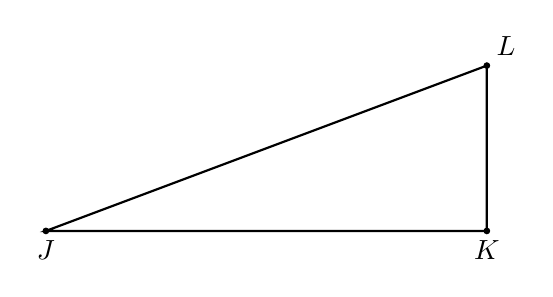
\begin{tikzpicture}[scale=0.7]
            \draw [thick](-1,0)--(7,0)--(7,3)--cycle;
            \draw [fill] (-1,0) circle [radius=0.05] node[below]{$J$};
            \draw [fill] (7,0) circle [radius=0.05] node[below]{$K$};
            \draw [fill] (7,3) circle [radius=0.05] node[above right]{$L$};
          \end{tikzpicture}
        \end{flushright}
        \item Solve the equation for $x=KL$. \vspace{3cm}
        \item Use the Pythagorean formula to find the length $JL$
      \end{enumerate}

\end{enumerate}
\end{document}